% %
% Computerised measurement books for effective public works accounting Ver-D1.0
%

\documentclass[twoside,a4paper]{refart}

\usepackage{longtable,tabu}
\usepackage{fancybox}
\usepackage[framemethod=tikz]{mdframed}
\usepackage{graphicx}
\usepackage{hyperref}

% mdframed options


% Remove top and bottom rules from maxipage
\maxipagerulefalse

% Framed block for screenshots and other formats
\newenvironment{fminipage}[1]%
{\begin{Sbox}\begin{minipage}{#1}\begin{center}}%
		{\end{center}\end{minipage}\end{Sbox}\shadowbox{\TheSbox}}

% note/attension environment
\newenvironment{noteblock}[1]%
{\begin{mdframed}[topline=false,bottomline=false, rightline=false,
		linewidth=2pt, frametitle={#1}]}%
		{\end{mdframed}}

\title{Computerised measurement books for effective public works accounting}
\author{Manu Varkey, CE\&MES \\
	Assistant Executive Engineer(Electrical) \\
	Central Public Works Department \\}

\date{25-07-2015, D1.0}

\pagestyle{myfootings}
\markboth{Computerised measurement books for effective public works accounting}%
{Computerised measurement books for effective public works accounting}

\makeindex 

\setcounter{tocdepth}{2}

\begin{document}
	
	\maketitle
	
	\begin{abstract}
		This document describes the use of computerised measurement books for maintaining an effective quantity account of public works. Emphasis is given to the recording of measurements and	routine preparation of bills using computerised techniques involving the \emph{CMB Automiser} software.
	\end{abstract}
	
	\tableofcontents
	
	\newpage
	
	
	%%%%%%%%%%%%%%%%%%%%%%%%%%%%%%%%%%%%%%%%%%%%%%%%%%%%%%%%%%%%%%%%%%%%
	
	\section{Introduction}
	
	 The government so as to meet the needs of the nation is required to carry out a number of public works. Most public works are executed under contract by qualified contractors winning competitive call of tenders. The contractor is bound by agreement with government to execute works in accordance with the terms and conditions of the agreement. After winning the tender and signing the agreement, the contractor proceeds to execute the work under the supervision of the engineer-in-charge in accordance with the schedule of quantities/B.O.Q and specifications stipulated in the agreement.
	 
	 \subsection{Quantity account of works}
	 
	 Quantity account of works records the detailed quantities of various schedule items contained in the agreement. The payments to contractors either as final payments for the entire work or as running account payments are made on the basis of the quantity account that have been recorded. In a public works set-up, the quantity account is maintained in the form of measurement books.
	 
	 \section{Measurement books}
	 
	 Measurement books are important records of public works which forms the basis of payments met out to contractors under the terms and conditions of the agreement. It is also a legal record based on which any disputes arising out of the contract are settled. Hence the proper maintenance of this record becomes imperative for both the contractor and the government official.
	 
	 Measurements relating to a work are recorded date wise in the order in which measurements are taken and if necessary in multiple measurement books. Any disputed items are also to be measured pending resolution. For making payments to contractors, an abstract of all measurements to be billed up to the preparation of the bill is compiled and up-to-date value of work done is obtained on the basis of the agreement rates, deviated item rates, extra/substituted item rates. Payment for the bill is made for the difference between up-to-date amount and the previous bill amount.
	 
	 \subsection{Computerised measurement books}
	 
	 Under the old procedure, the measurement books were recorded by the departmental supervisory staff in the presence of the contractor's representative. The bills will be submitted by the contractor based on this recorded measurements.
	 
	 Under revised rules, contractor himself is responsible for recording measurements in computerised measurement books (CMBs) and submission of bills/claims. The JE/AE/AEE will verify the measurements in the presence of the contractors/his authorised representative. 
	 
	 \subsection{General guidelines for the maintenance of CMBs}
	 
	 \begin{enumerate}
		 \item \attention The measurements shall be recorded and entered in computerised format by the contractor, and a hard copy shall be submitted to the Department. These measurements will then be checked by the JE/AE/AEE. At the time of bill preparation, the contractor shall incorporate all changes or corrections, done during the checks and submit to the department the corrected computerized measurements in the form of a book along with the draft measurement sheets.
		 \item The CMBs should be prepared at contractors cost in A4 size and hard bound in red colour. Pages shall be machine numbered.
		 \item Each page shall be initialled by the contractor/his representative. In case of the MB being signed by the contractor's representative, letter of authorisation shall be submitted along with the MB.
		 \item Number of pages shall be limited to 100. Any additional measurements should be made on a separate MB.
		 \item \attention The CMB number should be got alloted in advance from the division before recording measurements.
	 \end{enumerate}
	 
	 \subsection{Format of computerised measurement book}
	 
	 \subsubsection{Facing sheets}
	 
	 Following standard facing sheets should be added to the start of every CMB.
	 
	 \begin{enumerate}
		 	\item Certificate of AE/AEE as to the number of sheets in the CMB along with the CMB number, name of work, agreement number and agency.
		 	\item MB issue page.
		 	\item Page for recording remarks of officers conducting test check.
		 	\item Page for recording remarks of the accounts branch.
	 \end{enumerate}
	 
	 \subsubsection{Title block}
	 
	 A title block is of the format given below. It gives detailed description of the work whose measurements are being recorded.
	 
	 \begin{fminipage}{\textwidth}
	 	\begin{center}
	 		\textbf{DETAILS OF MEASUREMENTS} \\
	 	\end{center}
	 	
	 	\begin{longtabu}{p{.3\textwidth} c p{.5\textwidth}}
	 		Name of Work & : & \emph{\textless name of work\textgreater} \\
	 		Situation & : & \emph{\textless situation\textgreater}\\
	 		Agreement No. & : & \emph{\textless agreement number\textgreater}\\
	 		Agency & : & \emph{\textless agency}\\
	 		Date of Start & : & \emph{\textless actual date of start\textgreater}\\
	 		As per agreement & : & \emph{\textless date of start as per agreement\textgreater}\\
	 	\end{longtabu}
	 \end{fminipage}
	 
	 \subsubsection{Measurement group}
	 
	 Measurements are ordered according to the date of measurements. Each of these groups of measurements start with the block given below.
	 
	 \begin{fminipage}{\textwidth}
	 	\begin{longtabu}{p{.3\textwidth} c p{.5\textwidth}}
	 		Date of Completion & : & \emph{``work in progress"/ \textless completion date\textgreater} \\
	 		Date of Measurement & : & \emph{\textless date of measurement\textgreater} \\
	 		& & \\
	 	\end{longtabu}
	 \end{fminipage}
	 
	 \subsubsection{Measurements}
	 
	 \paragraph{Standard measurement item}
	 \label{item:standardmeasitem}
	 Standard format for the measurement item is given below. Most items of work can be recorded in the following format.
	 
	 \begin{maxipage}
	 	\begin{fminipage}{\textwidth}
	 		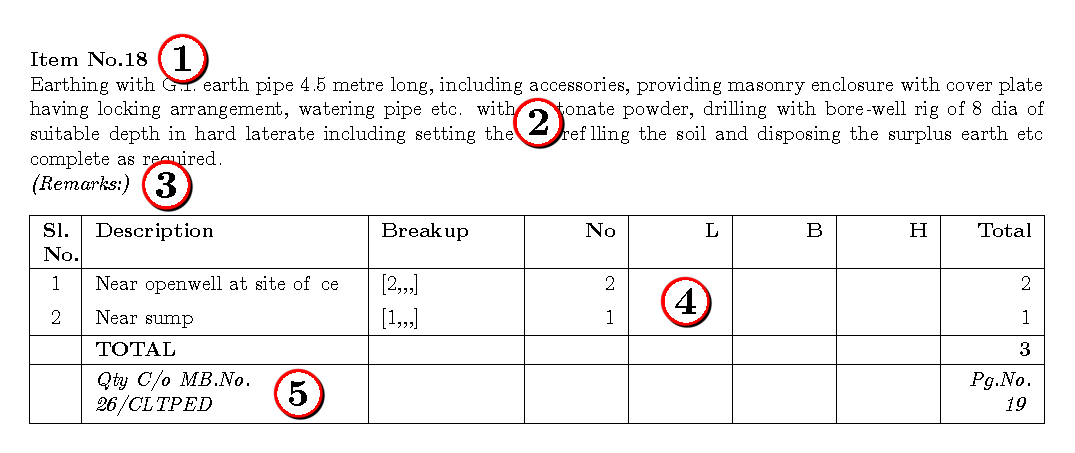
\includegraphics[width=1\linewidth]{figures/measurementstandard.pdf}
	 	\end{fminipage}
	 \end{maxipage}
	 
	 Essential features of the measurement item indicated by numbered markers in the above figure are described below.
	 
	 \begin{enumerate}
	 	\item Item number as per agreement schedule or extra/substituted/recovery item schedules. \\
	 	
	 	\begin{noteblock}{Note:}
	 		By convension extra items are denoted by E1, E2, E2.1 etc; Substituted items by S1, S2, S2.1 etc and recovery items by R1, R2, R2.1 etc
	 	\end{noteblock}
	 	
	 	\item Description as per agreement schedule or extra/substituted/recovery item schedules
	 	\item Any remarks about the item should go here.
	 	\item Tabulated list of measurements. The measurements are to be broken down into meaningful divisions which can be readily verified at site. Description should give the location (start and end locations in the case of lengths) where the item is being measured and should be easily identifiable at site. Breakup if applicable should be indicated for convenient checking of measurements. The total for each entry is obtained as $No \times Length \times Breadth \times Height$. The total for the measurement item is obtained as the sum of totals of individual entries.\\
	 	
	 	\begin{noteblock}{Examples:}
	 		\begin{small}
	 			\begin{longtabu} to \textwidth {X[1,c] X[10,l] X[5,l] X[1,r] X[1,r] X[1,r] X[1,r] X[1,r]}
	 				\hline
	 				\emph{Sl} & \emph{Description} & \emph{Breakup} & \emph{N} & \emph{L} & \emph{B} & \emph{H} & \emph{T} \\
	 				\hline
	 				\endhead
	 				1 & Inside room 1 of wing 2, 2nd floor & [1,,,] & 1 &  &  &  & 1\\ 
	 				2 & From SB7(Room1) to DB1(Room2) & [,1.5+15+ 1.5,,] &  & 18 &  &  & 18\\ 
	 				3 & From P1(near school building) to road crossing & [,15+14,,] &  & 29 &  &  & 29\\ 
	 			\end{longtabu}
	 		\end{small}
	 	\end{noteblock}
	 	
	 	\item Cross reference to the abstract of measurements where the item is billed. This should  indicate the serial number of the measurement book where the abstract is recorded and the page number in that measurement book where the item is carried over.
	 \end{enumerate}
	 
	 \paragraph{Special measurement items}
	 
	 The standard measurement item format may not be suitable for certain situations when the measurements are better understood in groups or for the measurement of electrical points, AC ducts etc which cannot be described conveniently using the standard measurement format. In such cases the essential structure of the measurement item may be modified while keeping all the essential features described above. Some of these are illustrated below.
	 
	 \begin{center}
	 	\begin{fminipage}{\textwidth}
	 		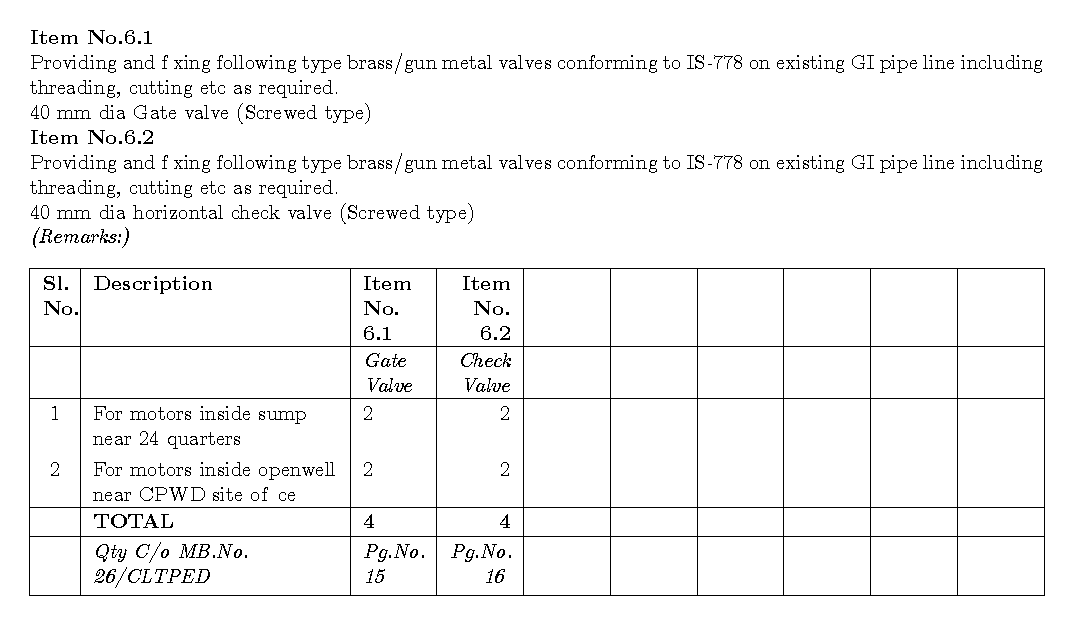
\includegraphics[width=1\linewidth]{figures/measurementNNNNNN.pdf}
	 	\end{fminipage}
	 \end{center}
	 
	 \begin{center}
	 	\begin{fminipage}{\textwidth}
	 		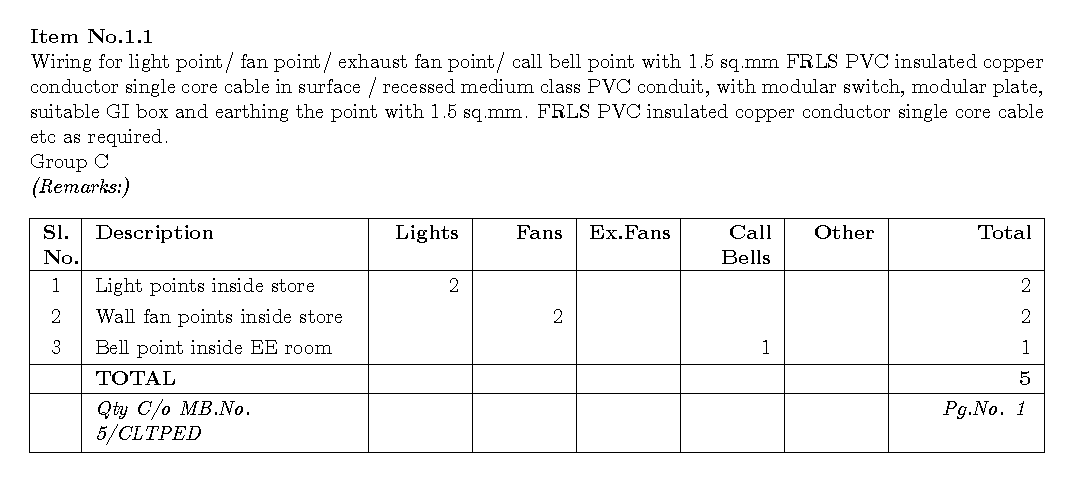
\includegraphics[width=1\linewidth]{figures/measurement_points.pdf}
	 	\end{fminipage}
	 \end{center}
	 
	 \begin{center}
	 	\begin{fminipage}{\textwidth}
	 		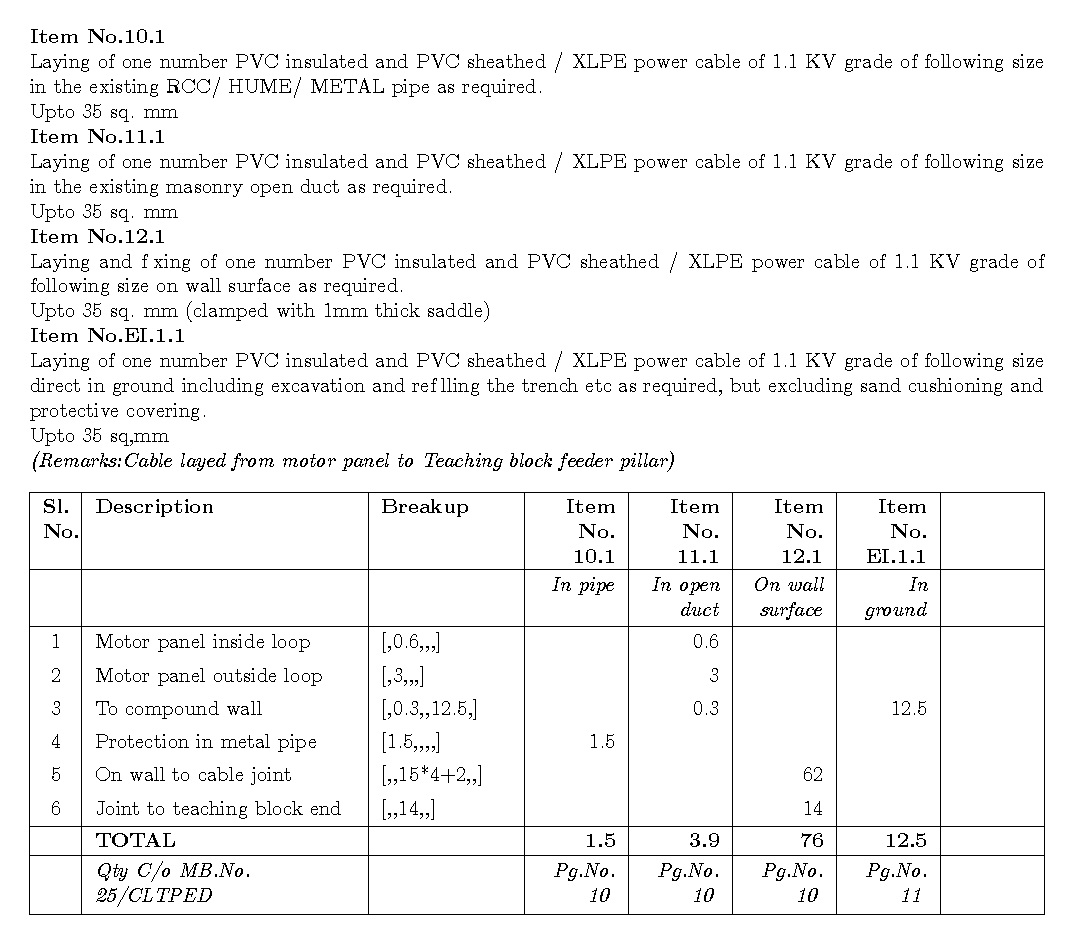
\includegraphics[width=1\linewidth]{figures/measurementLLLLL.pdf}
	 	\end{fminipage}
	 \end{center}
	 
	 \paragraph{Completion certificate}
	 
	 Standard completion certificate of the form given below should be included as the last item of the final measurement book recording measurements for the work.
	 
	 \begin{fminipage}{\textwidth}
	 	\begin{center}
	 		\bigskip
	 		\textbf{COMPLETION CERTIFICATE}
		 	\begin{longtabu}{p{.3\textwidth} c p{.5\textwidth}}
		 		Name of Work & : & \emph{\textless name of work\textgreater} \\
		 		Situation & : & \emph{\textless situation\textgreater}\\
		 		Agreement No. & : & \emph{\textless agreement number\textgreater}\\
		 		Agency & : & \emph{\textless agency}\\
		 		Date of Start & : & \emph{\textless actual date of start\textgreater}\\
		 		As per agreement & : & \emph{\textless date of start as per agreement\textgreater}\\
		 		Date of Completion & : & \emph{\textless date of completion\textgreater} \\
		 		&&
		 	\end{longtabu}
		 \end{center}
		 \parbox{0.9\linewidth}{
		 Certified that the work has been physically completed on \emph{\textbf{\textless date of completion\textgreater}} and that no defects are apparent and contractor has removed from the premises on which the work was carried out all the debris scaffolding and surplus materials and cleared off all dirt from wood work, ceiling, walls, floors and all other parts of the building up on which or about which he has been in possession for the purpose of execution thereof.
		 
		 This is however subject to measurement being recorded and quality being checked by the competent authority.
		 }\bigskip
	 \end{fminipage}
	 
	 \paragraph{Abstract of measurements}
	 For billing measurements, an abstract of measurements to be billed should be prepared in the format described. The agreement items should appear in the chronological order followed by extra item, substituted item and recovery items each appearing in the chronological order. 
	 
	 \attention
	 For each schedule item, the quantity of items should be carried forward from the last bill abstract (total item quantity in last bill) along with various measurements to be billed in this bill there by obtaining the up-to-date total quantity of measurements to be billed. (Last bill quantity + $\sum$(Quantity measured in this bill) = Total up-to-date quantity).
	 
	 Against the total quantity up-to-date, the full rates of items as per schedule and part rates allowed for the item are recorded along with total amount for the item ($Total = P.R \times Qty$)\\
	 
	 \begin{noteblock}{Note:}
	 	Quantity up to the deviation limit (30\% of agreement quantity) is billed at the agreement rate while quantities above that limit is billed at market rates. Therefore if the quantity to be billed exceeds deviation limit, then the quantity should be broken-down into that below deviation limit and that above deviation limit.
	 \end{noteblock}
	 
	 The individual totals for all the schedule items are summed up to obtain the total amount up-to this bill. Reducing the last bill amount from this total would give the amount of this bill since the previous bill.
	 
	 The structure of the abstract of measurements is illustrated below.
	 
	 \begin{center}
	 	\begin{fminipage}{\textwidth}
	 		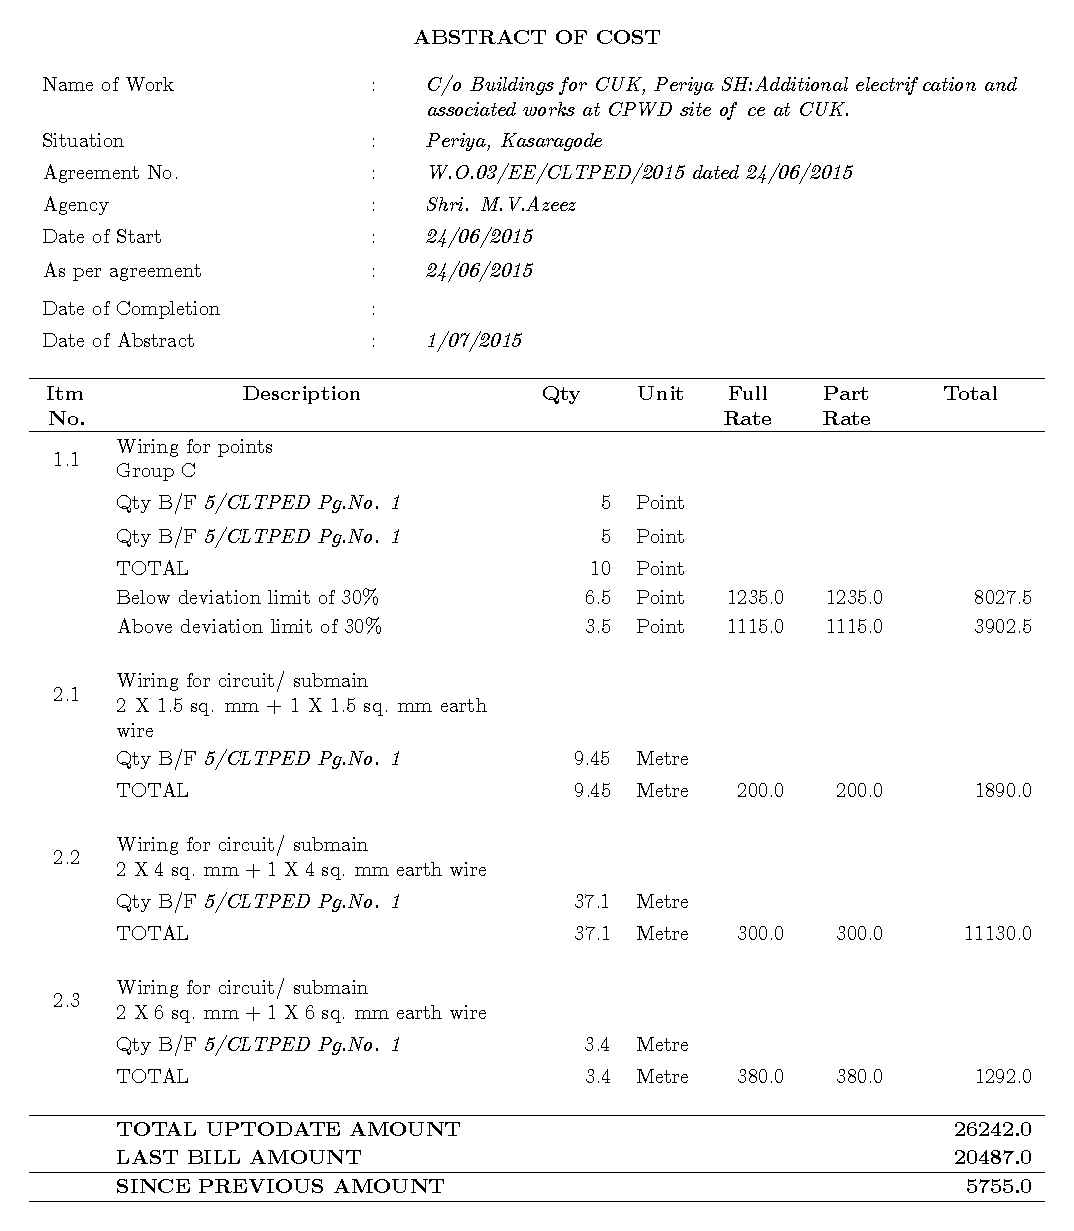
\includegraphics[width=1\linewidth]{figures/abstract.pdf}
	 	\end{fminipage}
	 \end{center}
	 
	 \begin{noteblock}{Note:}
	 	Two blank sheets should be added after the abstract for recording the pass and pay orders for the bill.
	 \end{noteblock}
	 
	 \subsection{Bill schedule and form}
	 Along with the measurement books, the contractor's claim is to be submitted in first and final bill form (CPWA-24) or the running account bill form (CPWA-26) in the case of running bills. The schedule attached to the bill should be of the following format.
	 
	 \begin{center}
	 	\begin{fminipage}{\textwidth}
	 		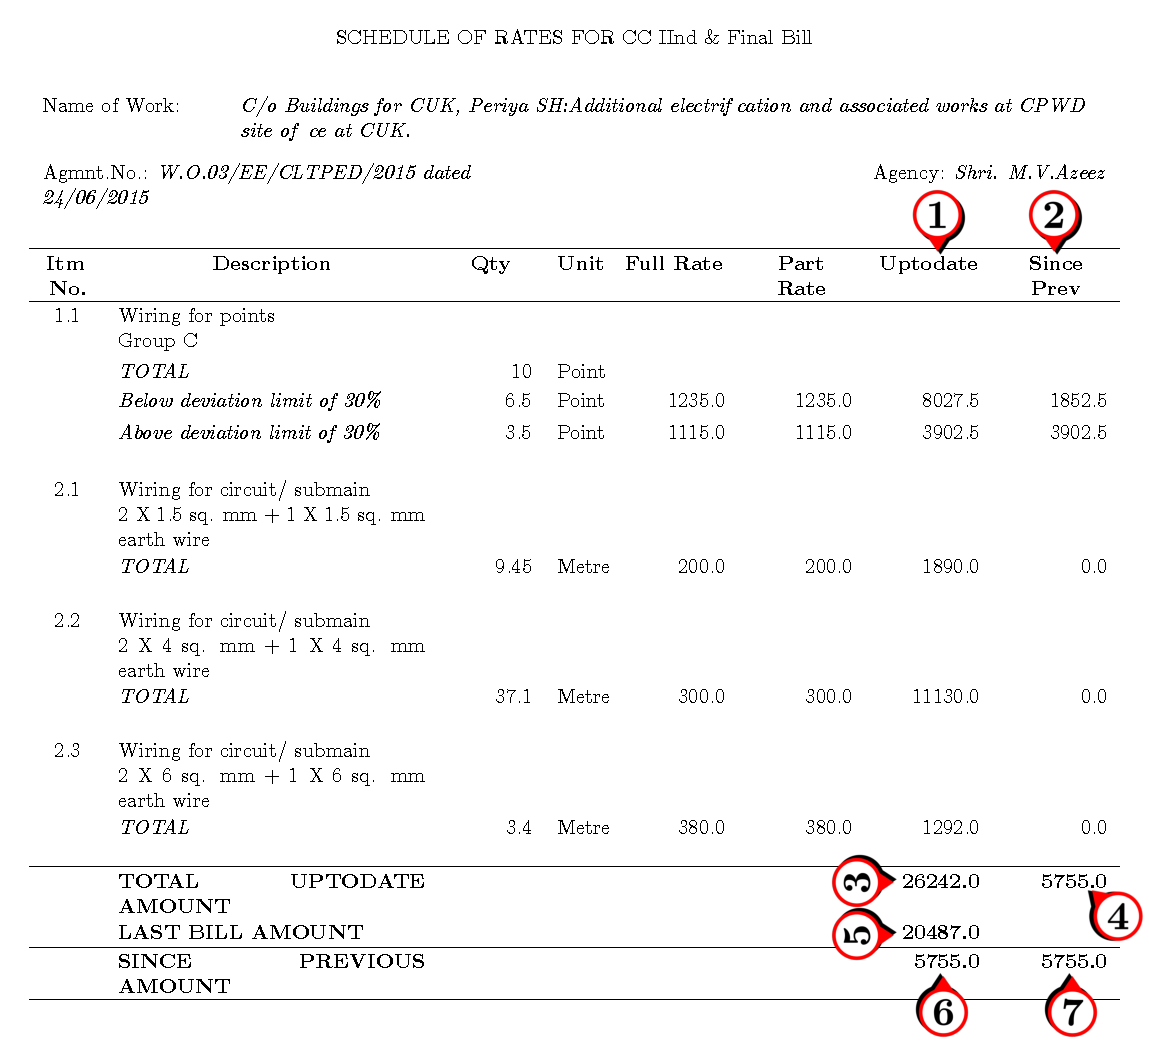
\includegraphics[width=1\linewidth]{figures/schedule.pdf}
	 	\end{fminipage}
	 \end{center}
	 
	 Essential features of the schedule indicated by numbered markers in the above figure are described below.
	 
	 \begin{enumerate}
	 	\item Upto date amount of item up-to this bill = Item Quantity $\times$ Item Part.Rate
	 	\item Amount of item in this bill - Amount of item in the previous bill (ie. column (1) of this bill - column (1) of last bill)
	 	\item Sum of Column (1)
	 	\item Sum of Column (2)
	 	\item Previous bill amount
	 	\item (5) - (3)
	 	\item (4) \\
	 \end{enumerate}
	 
	 \begin{noteblock}{Note:}
	 	Same value should be obtained for (6) and (7). Any discrepancy between the two values is an indication of arithmetic errors in the schedule.
	 \end{noteblock}
	 
	 \section{Computerised measurements using \emph{CMB Automiser}}
	 \emph{CMB Automiser} is a computer program which simplifies the recording of measurements and preparation of bills. It allows the user to perform these objectives with an intuitive interface and logical work flow. The results are presented in fully formatted, cross referenced \emph{pdf} documents.
	 
	 \subsection{Workflow}
	 
	 \begin{maxipage}
	 	\begin{center}
	 		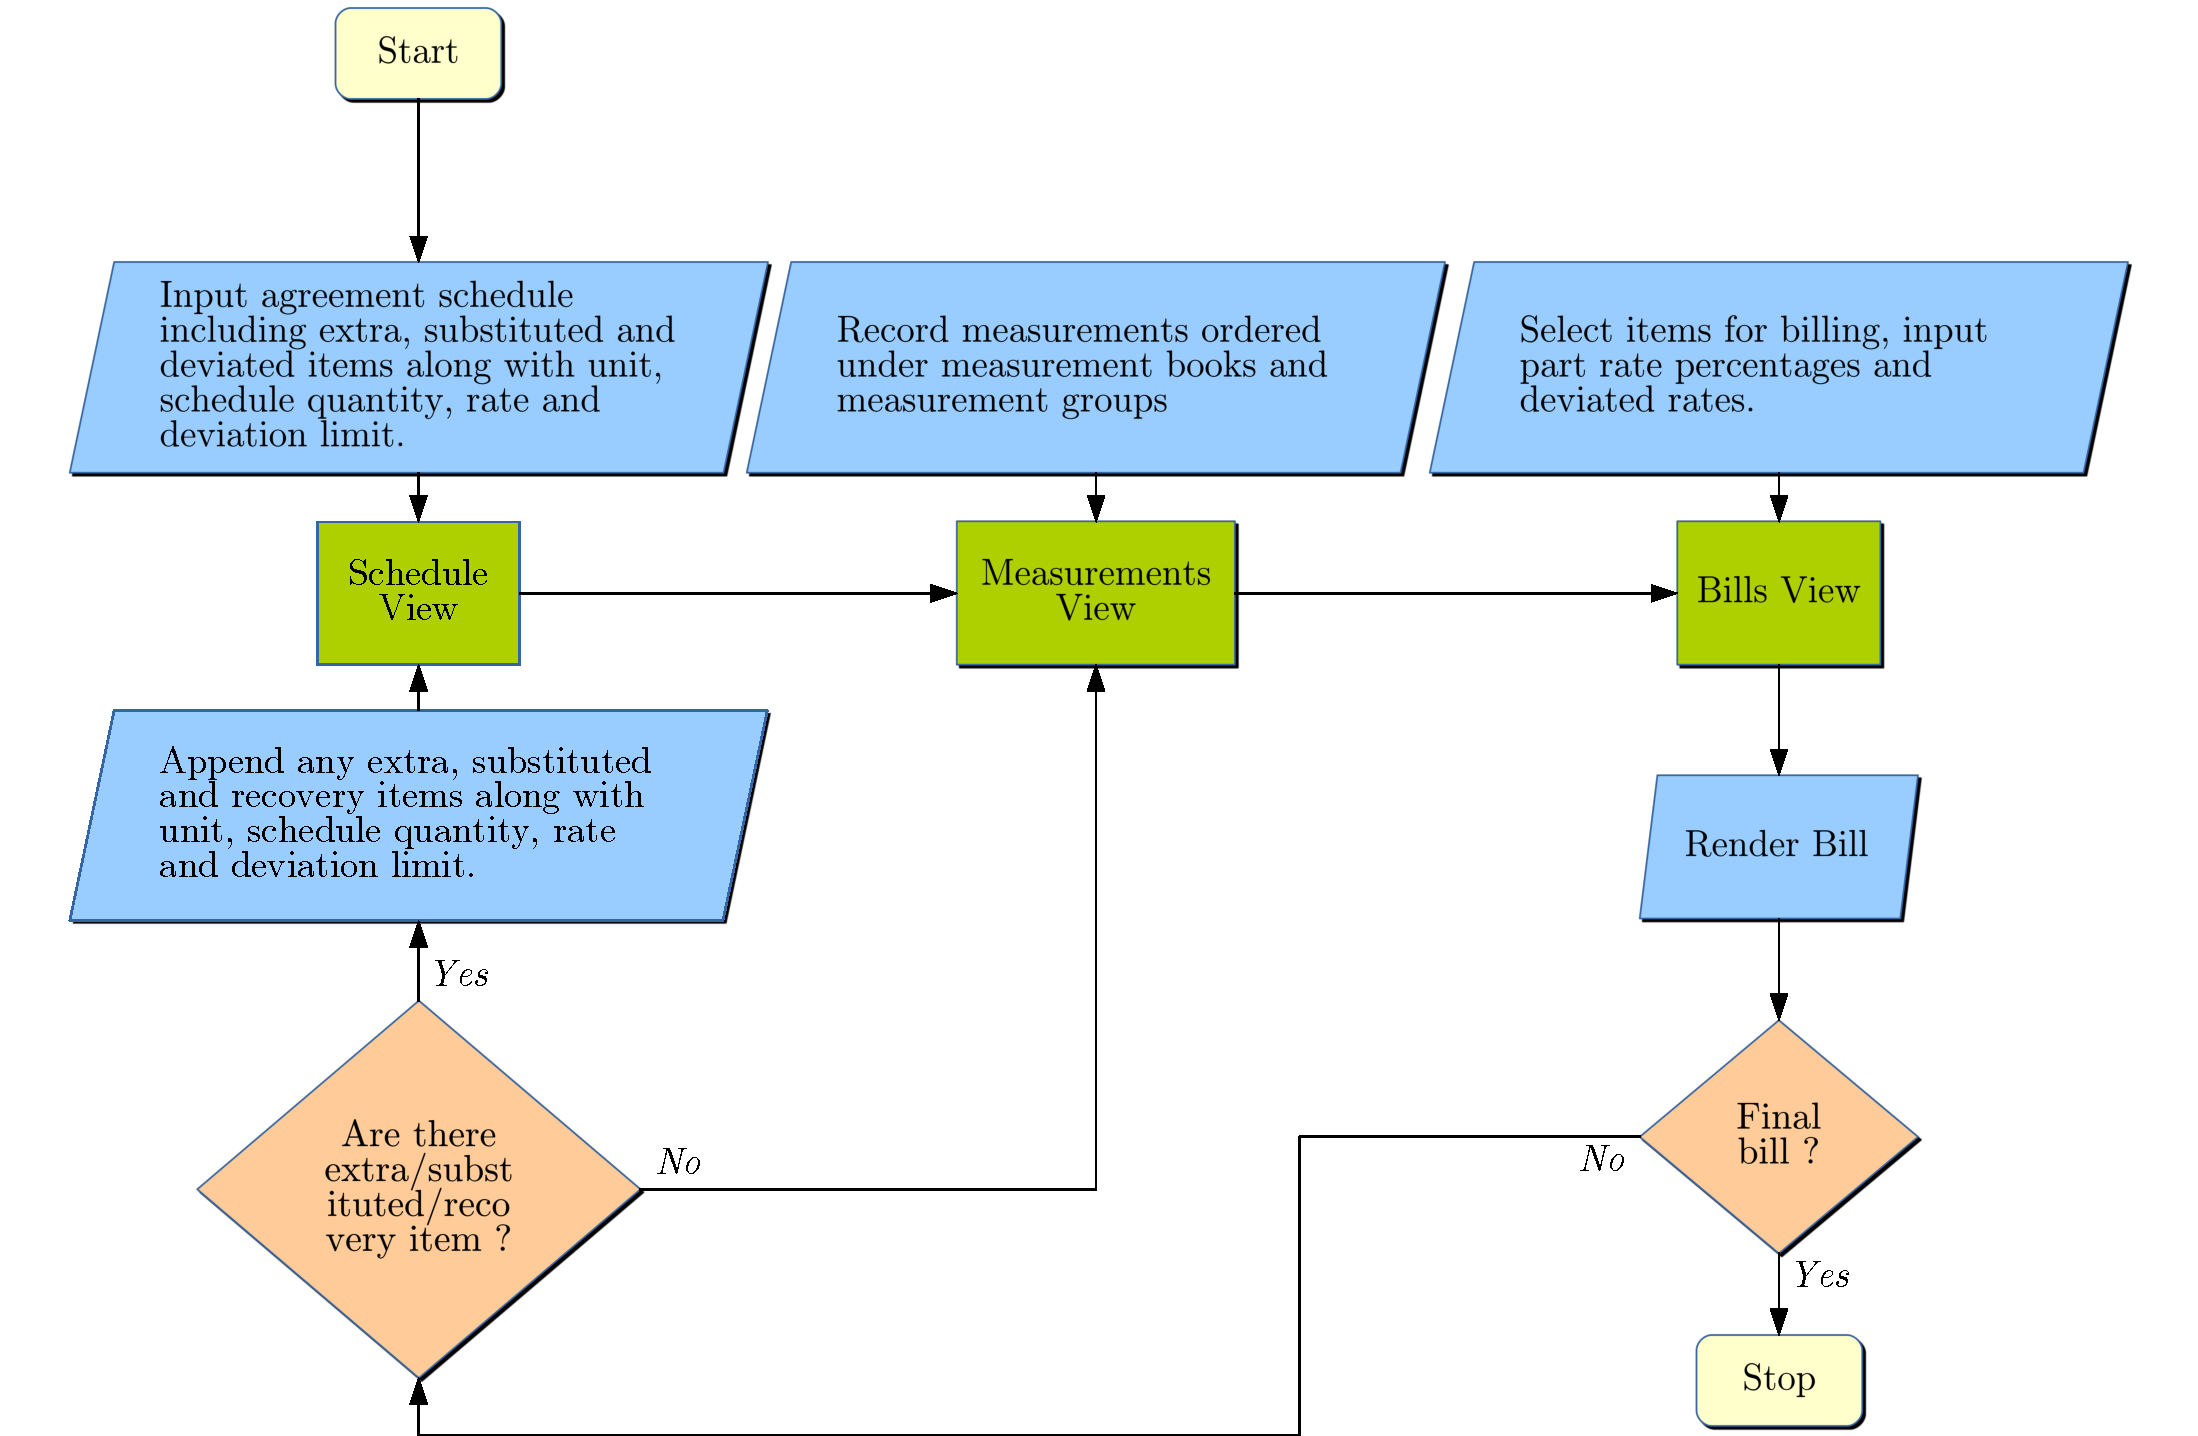
\includegraphics[width=1\linewidth]{figures/workflow.pdf}
	 	\end{center}
	 \end{maxipage}
	 
	 The program is organised in three tabs/views - \emph{schedule}, \emph{measurements} and \emph{bills} views. \emph{Schedule view} implements an interface to input the agreement schedule/import the schedule from a \emph{.xlsx} file. \emph{Measurements view} allows input/manipulation of details of CMBs and includes a number of convenient measurement item patterns. The \emph{Bill View} module allows billing of selected measurement items and implements part rates, excess rates for deviated items, custom previous bill support etc.
	 
	 Both CMBs and Bills can be rendered into a \emph{pdf} document from the respective modules. In addition \emph{Bill view} also allows export of final bill and deviation statement into a \emph{.xlsx} file for further processing.
	 
	 \subsection{Program Interface}
	 
	 \begin{center}
	 	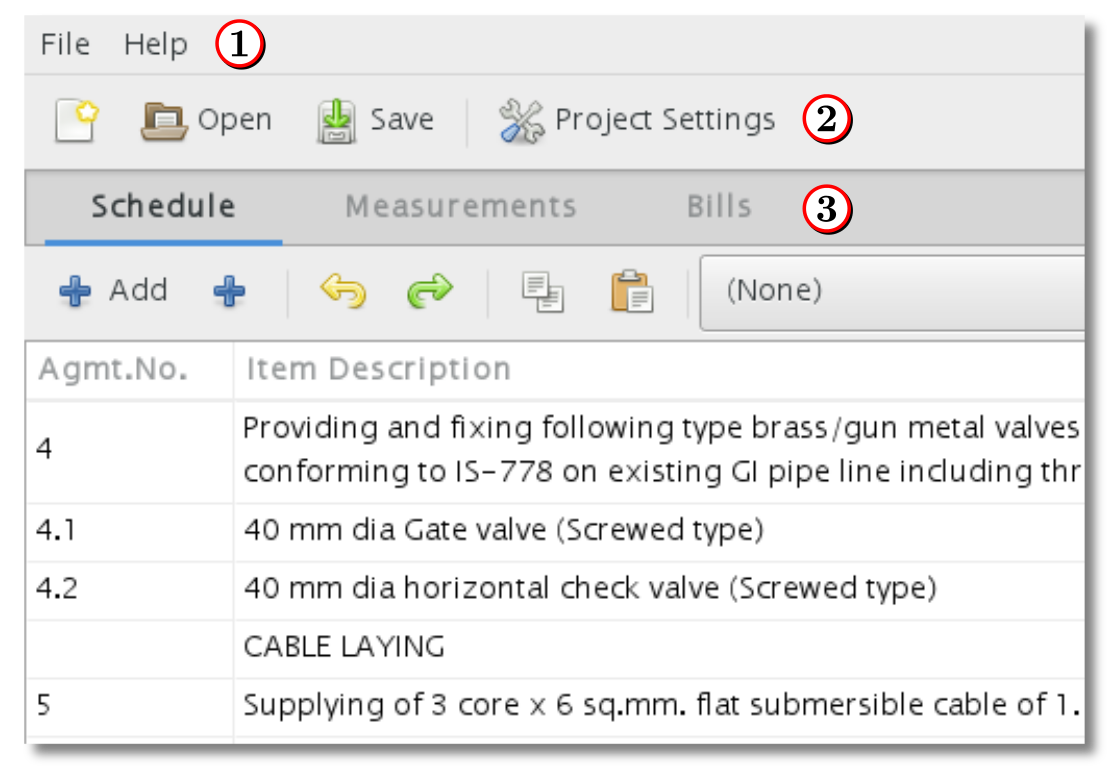
\includegraphics[width=1\linewidth]{screenshots/window_main.png}
	 \end{center}
	 
	 \emph{CMB Automiser} interface is divided into three components which are indicated by the numbered markers in the above figure. They are described below.
	 \begin{enumerate}
	 	\item Menu bar containing menu items for opening and saving projects as well as for opening a new program window. 
	 	\item Tool bar containing buttons for accessing commonly used functions. The Project settings can be accessed from here which allows the data related to the project to be entered.
	 	\item Tab bar for changing between Schedule, Measurements and Bills Views.
	 \end{enumerate}
	 
	 
	 
	 \subsection{Schedule View}
	 
	 \begin{maxipage}
	 	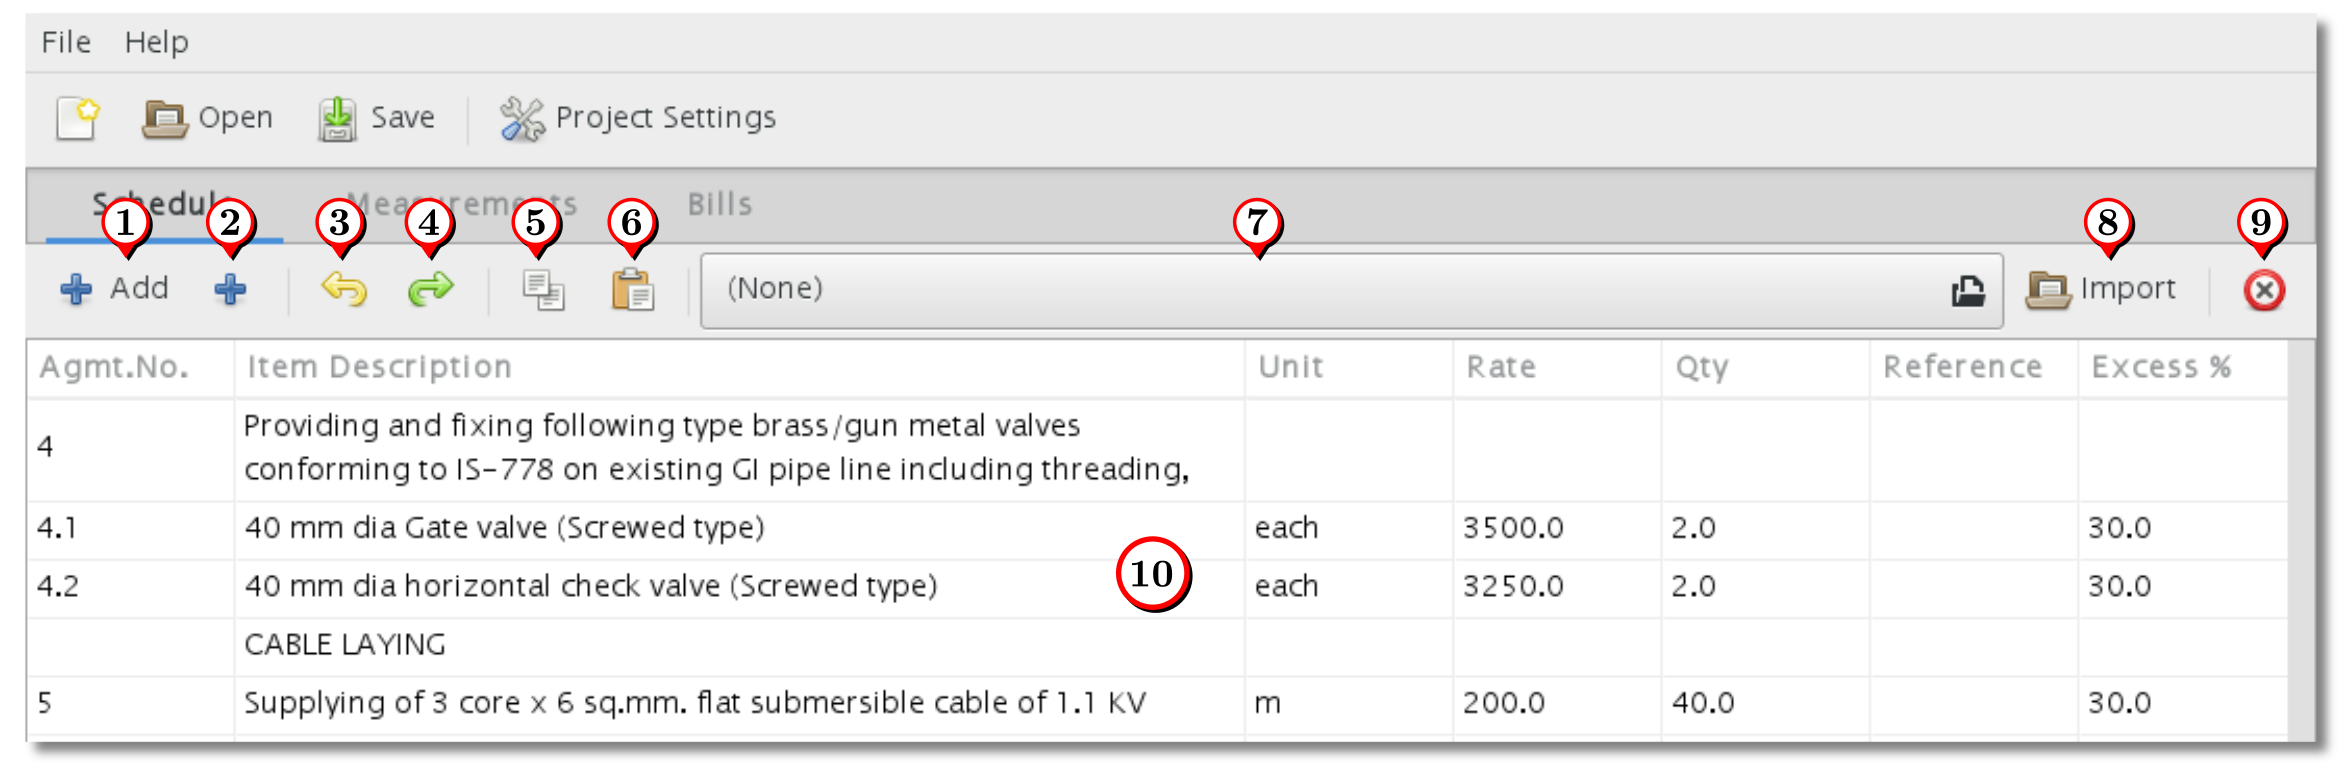
\includegraphics[width=1\linewidth]{screenshots/window_sch.png}
	 \end{maxipage}
	 
	 User interface elements indicated by numbered markers in the above figure are described below.
	 
	 \begin{enumerate}
	 	\item Add a blank entry in the schedule. If a schedule entry is selected, the entry will be inserted above the selected entry. If no entry is selected, the entry will be appended at the end.\\
	 	\begin{noteblock}{Tips!}
	 		Pressing \fbox{\emph{Esc}} will deselect all entries.
	 	\end{noteblock}
	 	\item Adds \emph{n} number of blanks entries in the schedule.
	 	\item Undo change. (\fbox{\emph{ctrl}} + \fbox{\emph{z}})
	 	\item Redo change. (\fbox{\emph{ctrl}} + \fbox{\emph{shift}} + \fbox{\emph{z}})	 
	 	\item Copy selected entries to clipboard.
	 	\item Paste entries into schedule. If a schedule entry is selected, the entries will be inserted above the selected entry. If no entry is selected, the entries will be appended at the end.
	 	\item Select a file for reading data.
	 	\item \attention Imports schedule entries from the selected file. Data can be read from \emph{.xlsx} files. This is the recommended method of entering data into schedule. The spreadsheet file should have data in the first sheet with columns in the same order as in the schedule list (10) and rows corresponding to the schedule items to be imported.\\
	 	\begin{noteblock}{Note:}
	 		If all entries in a file are not successfully imported into \emph{CMB Automiser}, it could mean that the file is damaged. This may also include some files downloaded from \emph{tenderwizard.com}. Such files can be repaired by opening the file in \emph{LibreOffice-Calc} and saving the file as a \emph{.xlsx} document.
	 	\end{noteblock}
	 	\item Removes selected entries from the schedule.
	 	\item The schedule list containing entries in the format Agmnt.No, Item Description, Unit, Rate, Quantity, Reference and Excess \%. \emph{Excess \%} denotes the percentage above which item will be billed at market rates. \attention While importing a document, if the \emph{Excess \%} column is left blank, it will default to 30\%.
	 \end{enumerate}
	 
	 \begin{noteblock}{Note:}
	 	After a bill has been added to the \emph{Bills view}, changing the structure of the schedule may mess up the bill. To prevent this from happening, all extra/substituted items to be added should be added at the end of the schedule.
	 \end{noteblock}
	 
	 \subsection{Measurements View}
	 
	 \begin{maxipage}
	 	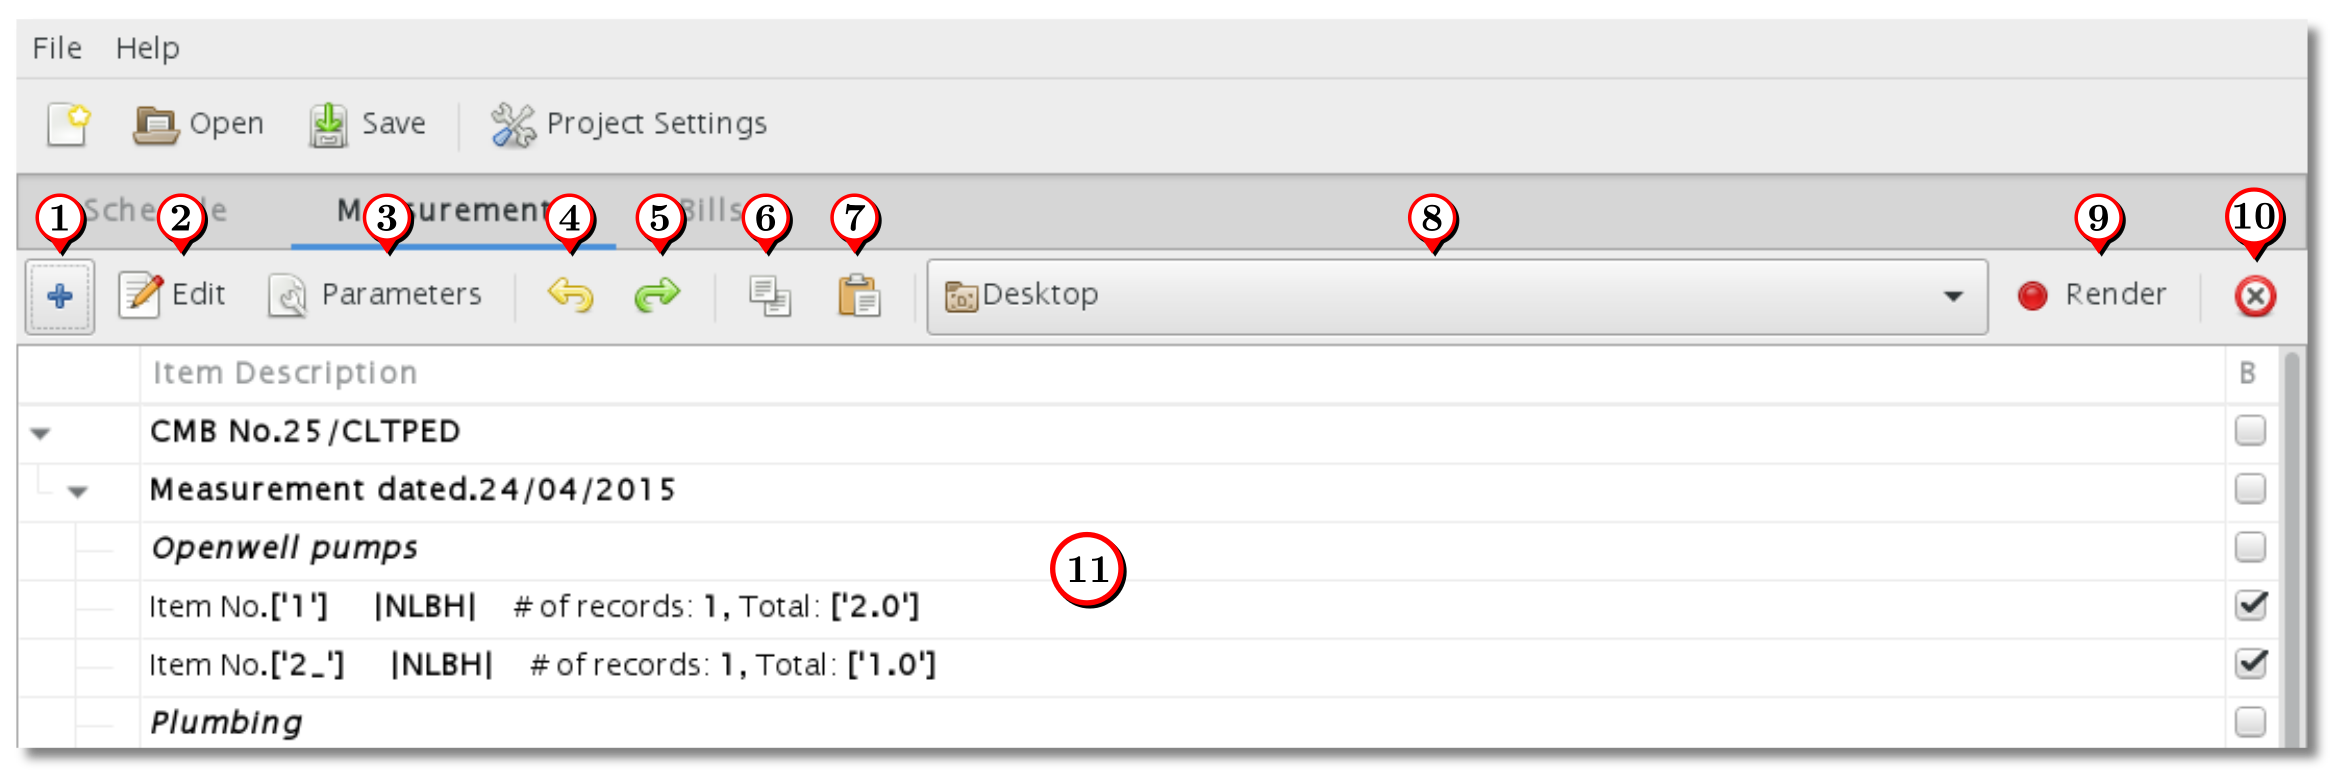
\includegraphics[width=1\linewidth]{screenshots/window_meas.png}
	 \end{maxipage}
	 
	 User interface elements indicated by numbered markers in the above figure are described below.
	 
	 \begin{enumerate}
	 	\item Opens menu for adding items to measurement list.
	 	\item Edit selected item.
	 	\item Edit parameters for the selected measurement item. \\
	 	\begin{noteblock}{Note:}
	 		Only some measurement items support parameters.
	 	\end{noteblock}
	 	\item Undo change. (\fbox{\emph{ctrl}} + \fbox{\emph{z}})
	 	\item Redo change. (\fbox{\emph{ctrl}} + \fbox{\emph{shift}} + \fbox{\emph{z}})	 
	 	\item Copy selected entries to clipboard.
	 	\item Paste entries into measurement list. If a measurement item is selected, the entries will be inserted above the selected entry. If no entry is selected, the entries will be appended at the end.
	 	\item Select a folder where the measurement book should be generated.
	 	\item Generates selected measurement book in the folder selected.
	 	\item Removes the selected entries from schedule.
	 	\item List of items organised in three tiers.
	 \end{enumerate}
	 
	 Measurement list follows a tree structure with items divided in three tiers as described below.
	 
	 \begin{enumerate}
	 	\item \textbf{CMB} (\fbox{\emph{$+$}} $\rightarrow$ \emph{CMB}) - Groups measurements under one measurement book. Takes the serial number of measurement book as parameter.
	 	\item \textbf{Measurement Group/Completion Certificate} - The second tier has two entries which can be added under the first tier (\emph{CMB}) as described below.
	 	\begin{enumerate}
	 		\item \textbf{Measurement Group} (\fbox{\emph{$+$}} $\rightarrow$ \emph{Measurement Group}) - Groups measurements under the date of measurement. Takes the measurement date as parameter.
	 		\item \textbf{Completion Certificate} (\fbox{\emph{$+$}} $\rightarrow$ \emph{Completion Certificate}) - Inserts a completion certificate to the measurement book. Takes the completion date as parameter.
	 	\end{enumerate}
	 	\item \textbf{Measurement Items} - Measurement items are added under a \emph{Measurement Group}. It records  measurements in one of the various formats. There is also a special item for inserting a heading.
	 \end{enumerate}
	 
	 \begin{noteblock}{Note:}
	 	A \emph{CMB} item should be present and selected before adding a \emph{Measurement Group}. Similarly a \emph{Measurement Group} should be present and selected before adding a \emph{Measurement Item}.
	 \end{noteblock}
	 
	 \subsubsection{Measurement Items}
	 
	 Some of the most frequently used measurement items are discussed below.
	 
	 \paragraph{Heading} (\fbox{\emph{$+$}} $\rightarrow$ \emph{Heading}) - Inserts a text entry in the measurement book which may be used to logically separate measurements.
	 
	 \paragraph{Item NLBH} \label{item:measitemnlbh} (\fbox{\emph{$+$}} $\rightarrow$ \emph{Item NLBH}) - Records measurements in the standard format given in \ref{item:standardmeasitem}. On adding the item, the following measurement entry form pops up allowing entry of measurements and other particulars.
	 
	 \begin{maxipage}
	 	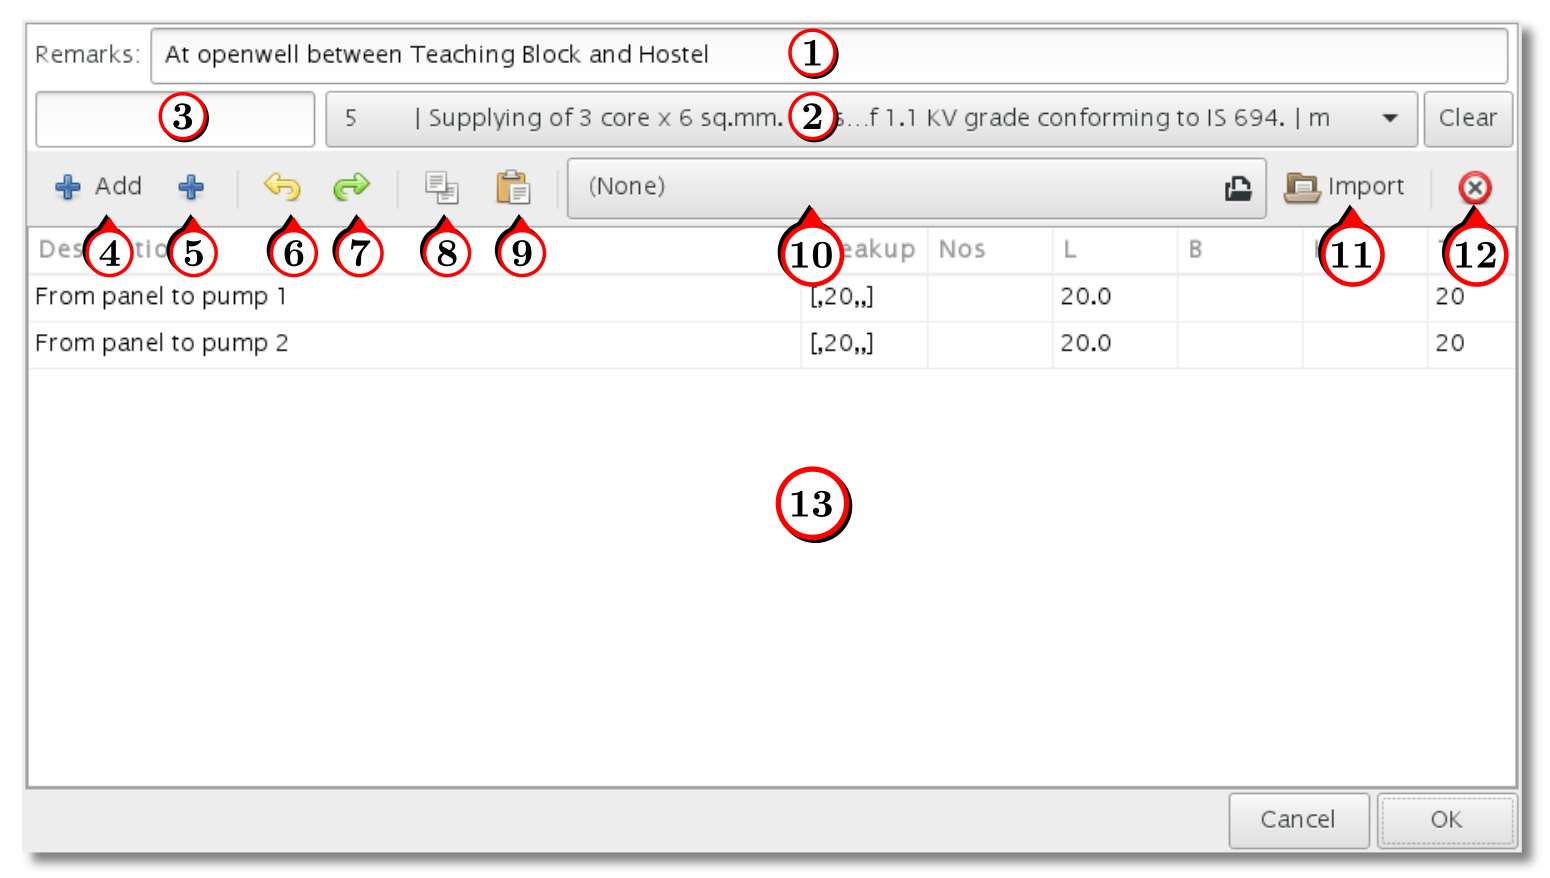
\includegraphics[width=1\linewidth]{screenshots/window_nlbh.png}
	 \end{maxipage}
	 
	 User interface elements indicated by numbered markers in the above figure are described below.
	 
	 \begin{enumerate}
	 	\item Any remarks about the measurement should go over here.
	 	\item Schedule item corresponding to the measurement should be selected from the drop-down menu.\\
	 	\begin{noteblock}{Note:}
	 		For items spanning multiple rows, the last row containing the rate and quantity should be selected. This row should have an \emph{Agmnt.No.} associated with it for proper functioning of the program. If it is not there a suitable derivative of the agreement number can be used (For example: the last row of item number \emph{7.5} can be numbered \emph{7.5\_}).
 		\end{noteblock}
 		\item Short abbreviation of the item being measured in 2 or 3 words (For example: 3x4, Cable on wall, Cable in trench etc.) for easy identification.
	 	\item Adds a blank row in the measurement. If a row is selected, the blank row will be inserted above the selected row. If no row is selected, the row will be appended at the end.\\
	 	\begin{noteblock}{Tips!}
	 		\begin{itemize}
		 		\item Pressing \fbox{\emph{Ctrl}} will deselect all rows.
		 		\item Cycle through rows horizontally using \fbox{\emph{Tab}} / \fbox{\emph{Shift}}+\fbox{\emph{Tab}} (forward/backward).
		 		\item Cycle through rows vertically using \fbox{\emph{Enter}} / \fbox{\emph{Shift}}+\fbox{\emph{Enter}} (up/down).
	 		\end{itemize}
	 	\end{noteblock}
	 	\item Adds \emph{n} number of blank rows in the measurement.
	 	\item Undo change. (\fbox{\emph{ctrl}} + \fbox{\emph{z}})
	 	\item Redo change. (\fbox{\emph{ctrl}} + \fbox{\emph{shift}} + \fbox{\emph{z}})	 
	 	\item Copy selected rows to clipboard.
	 	\item Paste rows into the measurement item. If a row is selected, the copied rows will be inserted above the selected row. If no row is selected, the rows will be appended at the end.
	 	\item Select a file for reading data.
	 	\item Imports measurement rows from the selected file. Data can be read from \emph{.xlsx} files. The spreadsheet file should have data in the first sheet with columns in the same format as the measurement items and rows corresponding to the measurement rows to be imported.\\
	 	\item Removes the selected rows from the measurement schedule.
	 	\item The measurement list has columns in the format Description, No, Length, Breadth, Height and Total. The total is obtained as $No \times Length \times Breadth \times Height$. Any zero value is omitted from the product. The total for the measurement item is obtained as the sum of totals of individual rows. The values entered can also be simple mathematical formulas (for ex: $1+3+1.5*2$). This will be displayed in the breakup column.
	 \end{enumerate}
	 
	 \paragraph{Item LLLLL} (\fbox{\emph{$+$}} $\rightarrow$ \emph{Item LLLLL}) - Allows recording measurements of up-to five linear items with breakup displayed. Measurement entry form is of the following format.
	 
	 \begin{maxipage}
	 	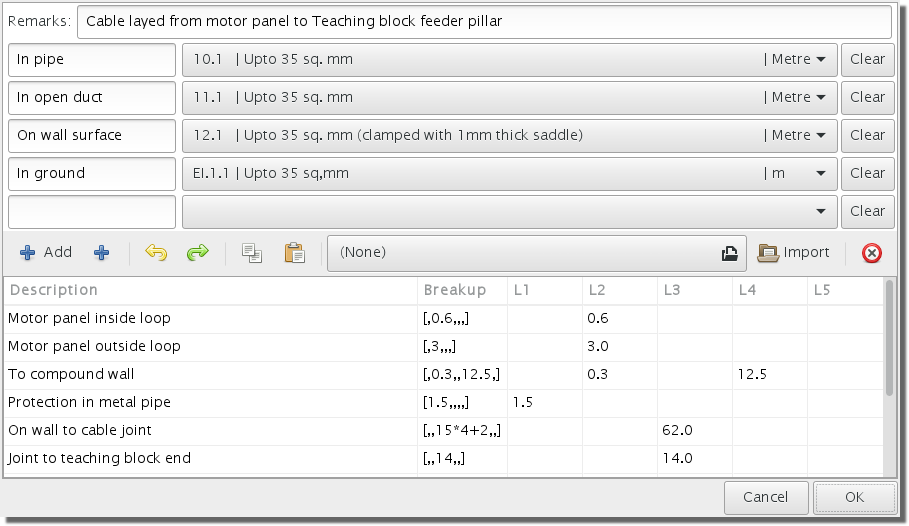
\includegraphics[width=1\linewidth]{screenshots/window_lllll.png}
	 \end{maxipage}
	 
	 The entry form is identical to that described in \ref{item:measitemnlbh}. The only difference is the addition of multiple schedule item selection boxes corresponding to the five items being measured. The text entries corresponding to each schedule item allows for entering short abbreviations for the items being measured in 2 or 3 words (For example: 3x4, Cable on wall, Cable in trench etc.) for easy identification of the item being measured. These abbreviations will be displayed on top of the column corresponding to the items being measured in the generated measurement book.
	 
	 The measurement list has columns in the format Description, Breakup, Item 1, Item 2, Item 3, Item 4 and Item 5. The total for each of the five items is obtained as the sum of the corresponding cells in each row.
	 
	 \paragraph{Item NNNNNNNN} (\fbox{\emph{$+$}} $\rightarrow$ \emph{Item NNNNNNNN}) - Allows recording measurements of up-to eight countable items. Unlike \emph{Item LLLLL}, no breakup of items is displayed.
	 
	 The measurement list has columns in the format Description, Item 1, Item 2, Item 3, ..., Item 8. The total for each of the eight items is obtained as the sum of the corresponding cells in each row.
	 
	 \paragraph{Item nnnnnT} (\fbox{\emph{$+$}} $\rightarrow$ \emph{Item nnnnnT}) - Allows recording measurements of single item. No breakup is displayed.
	 
	 The measurement list has entries in the format Description, Item 1, Item 2, Item 3, ..., Item 5 and Total. The total for each row is obtained as $Item1 + Item2 + ... + Item 5$. The total for the measurement item is obtained as the sum of totals of individual rows.
	 
	 \paragraph{Elec: Table of Points} (\fbox{\emph{$+$}} $\rightarrow$ \emph{Elec: Table of Points}) This item is a derivative of \emph{Item nnnnnT} suitable for measuring electrical points. The item has column headers in the format Light points, Fan Points, Ex. Fan points, Call bell points, Other points and Total Points.
	 
	 \subsection{Bills View}
	 
	 \begin{maxipage}
	 	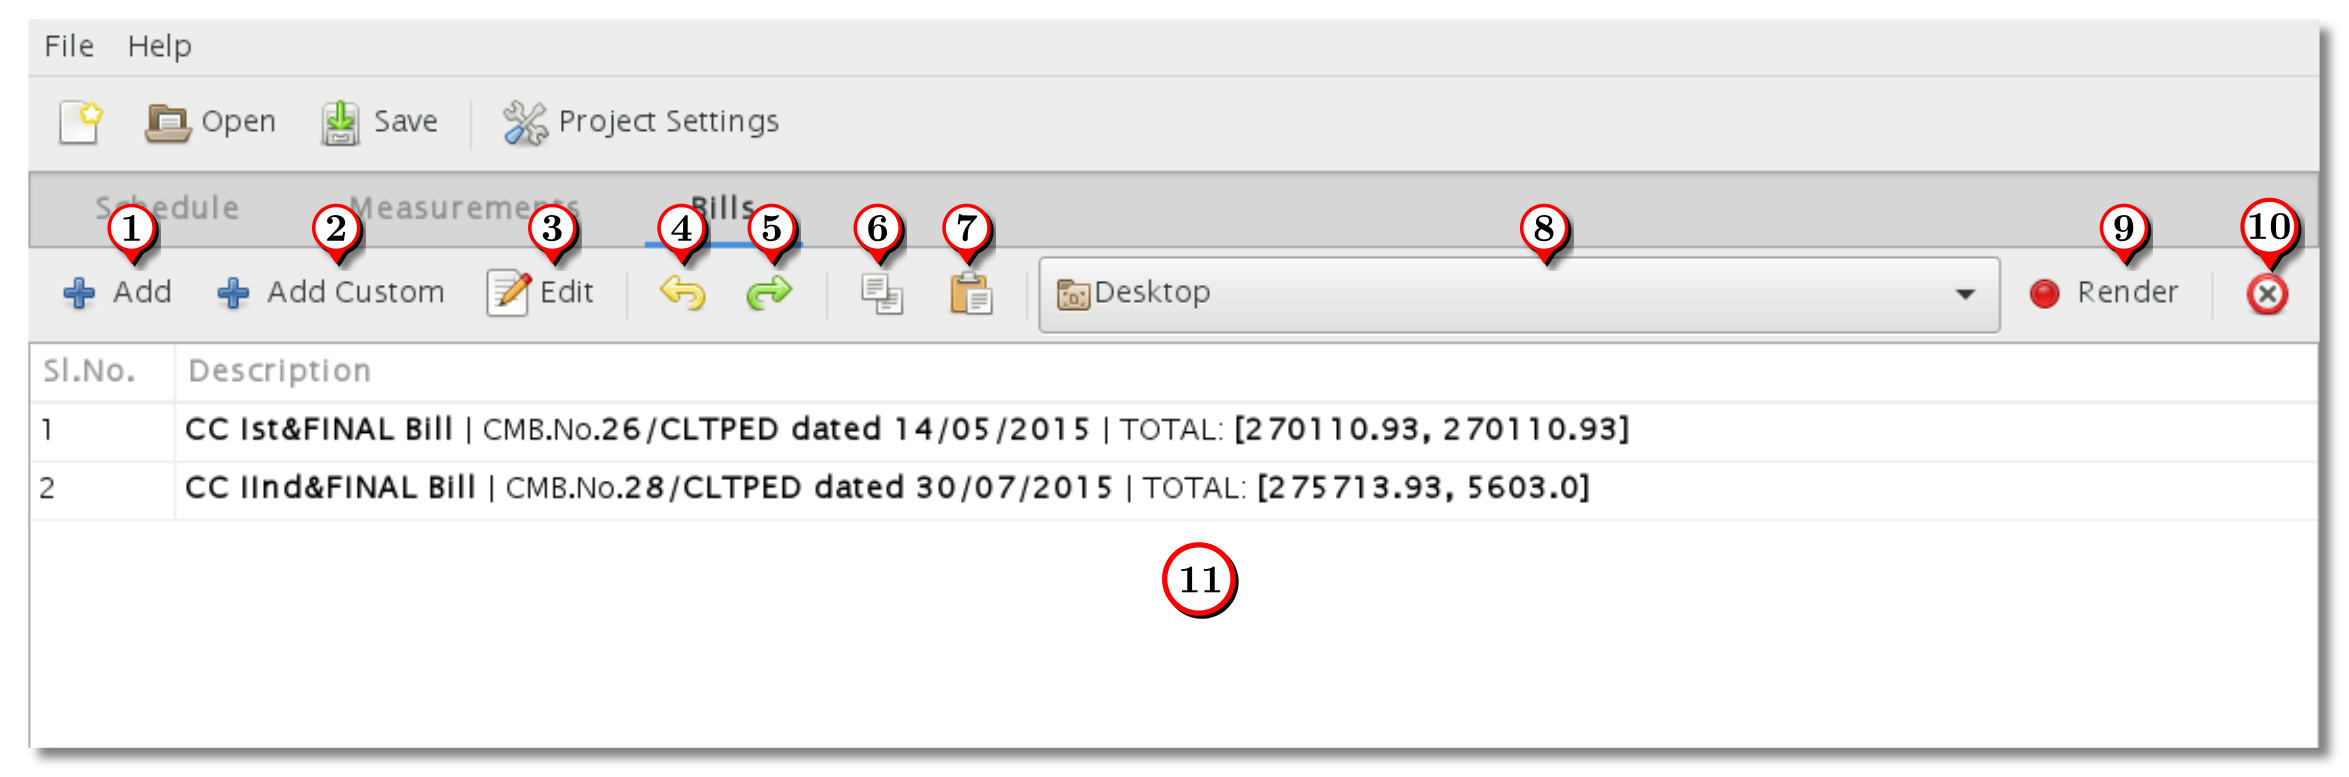
\includegraphics[width=1\linewidth]{screenshots/window_bill.png}
	 \end{maxipage}
	 
	 User interface elements indicated by numbered markers in the above figure are described below.
	 
	 \begin{enumerate}
	 	\item Adds a new bill to the bill list.
	 	\item Adds a new \emph{Custom bill} to the bill list. This option is used to carry forward values from a bill not prepared using \emph{CMB Automiser}
	 	\item Edit the selected bill.
	 	\item Undo change. (\fbox{\emph{ctrl}} + \fbox{\emph{z}})
	 	\item Redo change. (\fbox{\emph{ctrl}} + \fbox{\emph{shift}} + \fbox{\emph{z}})	 
	 	\item Copy selected bill to clipboard. Only bill title, MB name, bill date, part rate percentages and deviated item rates are copied.
	 	\item Paste bill. If a bill is selected, this bill will be overwritten. If no bill is selected, a new bill will be generated at the end from the copied values.
	 	\item Select a folder where the bill should be generated.
	 	\item Generates selected bill and associated measurement books in the folder selected.
	 	\item Delete the selected bill.
	 	\item List of bills.
	 \end{enumerate}
	 
	 \subsubsection{Billing Measurements}
	 
	 On selecting the \emph{Add} option from Bills view, the following window will pop-up allowing selection of the measurement items to be billed. A measurement can be selected for billing by ticking the check-box to the right of the item. Items selected for billing in the current bill are displayed in Blue colour. Other details about the bill like Title, CMB name, and date can also be filled in. The previous bill can be selected from the drop-down menu provided. The quantities corresponding to the previous bill will be carried over automatically if it is selected. For first RA/Final bill, this option should be set to \emph{None}.\\
	 
	 \begin{maxipage}
	 	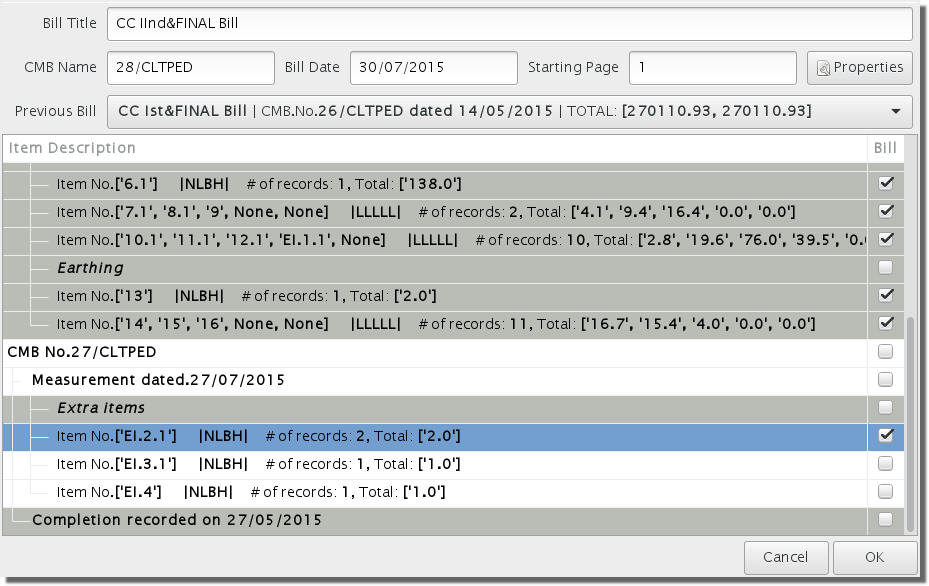
\includegraphics[width=1\linewidth]{screenshots/window_bill_edit.png}
	 \end{maxipage}
	 
	 \begin{noteblock}{Note:}
	 	The starting page number option allows the abstract to be generated in the same measurement book as the one containing the measurements being billed. This can be achieved by setting the same CMB name and setting the starting page as one above the number of pages in the measurement book containing the measurements being billed. In all other cases it should be set to 1.
	 \end{noteblock}
	 
	 \paragraph{Bill Properties}
	 
	 On selecting the \emph{Properties} button the following dialog window pops-up allowing the entry of part rate percentages (Column \emph{P.R.(\%)} for below deviation limit and Column \emph{Excess P.R.(\%)} for above deviation limit) and deviated item rates (Column \emph{Excess Rate}) corresponding to each item of the schedule. The column \emph{Excess?} gives indication whether an item has exceeded the deviation limit.
	 
	 \begin{maxipage}
	 	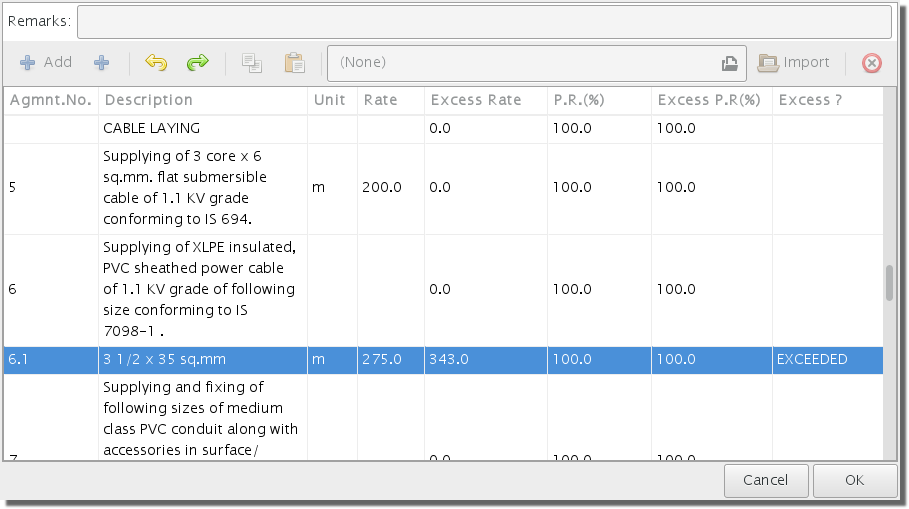
\includegraphics[width=1\linewidth]{screenshots/window_bill_prop.png}
	 \end{maxipage}
	 
	 \subsubsection{Adding a custom bill}
	 
	 \attention The custom bill option is used if the previous bill of a particular bill was not prepared using \emph{CMB Automiser}. In such cases, the bill to be selected as the previous bill should first be prepared using the custom bill option. On selecting the option from \emph{Bills view}, a window similar to regular bill will pop-up with section allowing selection of the measurement items disabled. Other details about the bill like Title, CMB name, and date can be filled in.\\
	 
	 \paragraph{Bill Properties}
	 
	 On selecting the \emph{Properties} button the following dialog window pops-up allowing the entry of total quantity (Column \emph{Total Qty}), Amount below deviation limit (Column \emph{Amount}) and Amount above deviation limit  (Column \emph{Excess Amount}) corresponding to each item of the schedule.
	
	 \begin{maxipage}
	 	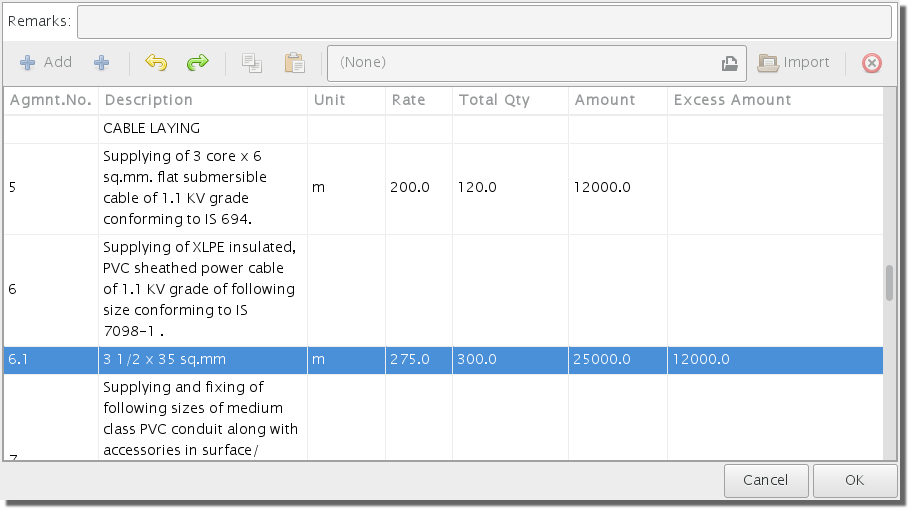
\includegraphics[width=1\linewidth]{screenshots/window_bill_cust_prop.png}
	 \end{maxipage}
	 
	 \emph{Custom bills} appear in red colour in the bills view. After addition, it can be selected as the previous bill just like the normal bill.
	 
	 \section{Conclution}
	 
	 This article was an attempt to introduce the basics of quantity accounting used in public works organisations especially in the central public works division. Detailed description of the recording of measurements in general and computerised techniques using \emph{CMB Automiser} was presented. This document was also written with the purpose of serving as a manual for \emph{CMB Automiser}. 
	 
	 The use of computerised accounting techniques if implemented orderly can simplify and expedite procedures. This will allow the execution staff to rightly concentrate on technical issues rather than on clerical work which is better delegated to those more competent in it.
	 
\end{document}